\section{Luthfi Muhammad Nabil(1174035)}
\subsection{Mencoba LeafletJS}
LeafletJS merupakan library yang dapat menambahkan penanda ke peta yang nantinya dapat diubah oleh developer. Berikut implementasinya : 
\begin{enumerate}
    \item Jalankan mapproxy terlebih dahulu
    \hfill\break
    \begin{figure}[H]
        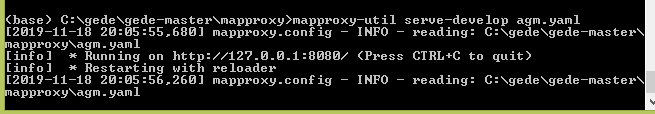
\includegraphics[width=8cm]{figures/1174035/tugas5/1.png}
        \centering
        \caption{Menjalankan map proxy}
    \end{figure}
    \item Buat file baru dengan ekstensi HTML
    \hfill\break
    \begin{figure}[H]
        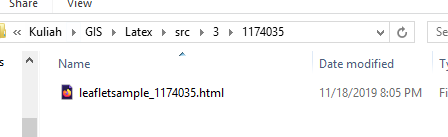
\includegraphics[width=8cm]{figures/1174035/tugas5/2.png}
        \centering
        \caption{Membuat file html}
    \end{figure}
    \item Isi tag head dengan kode berikut
    \lstinputlisting[firstline=2, lastline=9]{src/3/1174035/leafletsample_1174035.html}
    \item Isi tag body dengan kode berikut
    \lstinputlisting[firstline=10, lastline=19]{src/3/1174035/leafletsample_1174035.html}
    \item Lalu coba buka file html tersebut dan coba lihat hasilnya
    \hfill\break
    \begin{figure}[H]
        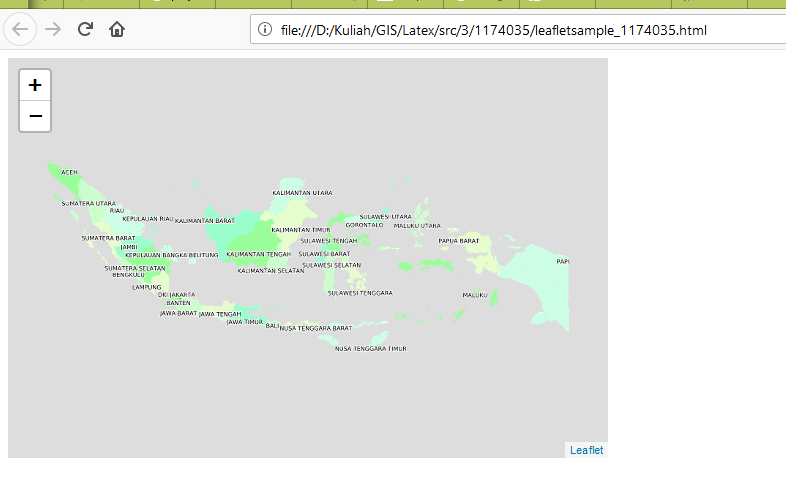
\includegraphics[width=8cm]{figures/1174035/tugas5/3.png}
        \centering
        \caption{Mencoba file HTML}
    \end{figure}
    \item Lalu untuk menambahkan beberapa sampel marker, coba dengan menggunakan sintaks berikut : 
        \break
        \begin{itemize}
            \item Marker \break Untuk mencoba menggunakan marker, silahkan coba dengan kode berikut
            \lstinputlisting[firstline=22, lastline=22]{src/3/1174035/leafletsample_1174035.html}
            \hfill\break
            \begin{figure}[H]
                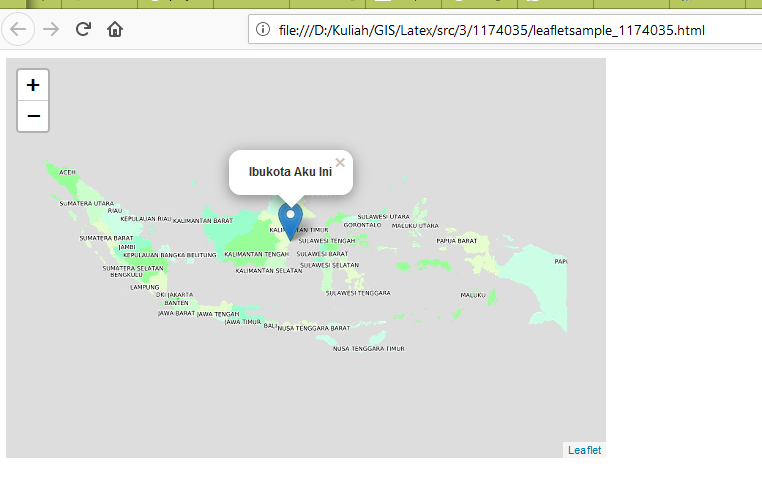
\includegraphics[width=8cm]{figures/1174035/tugas5/4.png}
                \centering
                \caption{Mencoba marker}
            \end{figure}
            \item Circle \break Untuk mencoba menggunakan circle, silahkan coba dengan kode berikut
            \lstinputlisting[firstline=24, lastline=28]{src/3/1174035/leafletsample_1174035.html}
            \hfill\break
            \begin{figure}[H]
                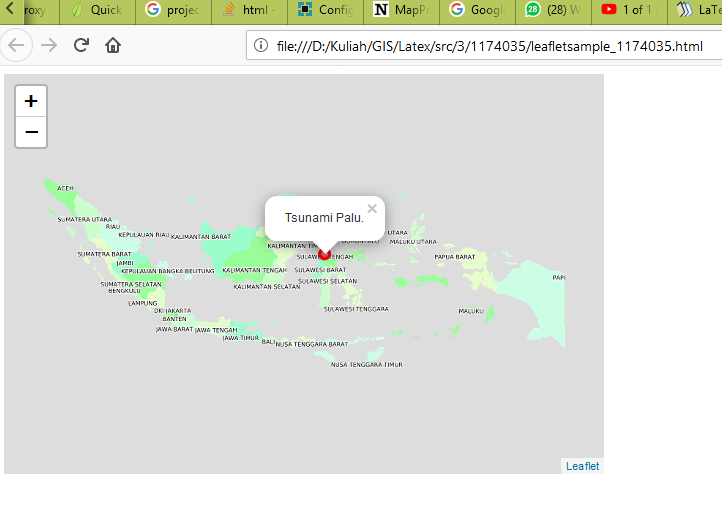
\includegraphics[width=8cm]{figures/1174035/tugas5/5.png}
                \centering
                \caption{Mencoba Circle}
            \end{figure}
            \item Polygon \break Untuk mencoba menggunakan polygon, silahkan coba dengan kode berikut
            \lstinputlisting[firstline=29, lastline=34]{src/3/1174035/leafletsample_1174035.html}
            \hfill\break
            \begin{figure}[H]
                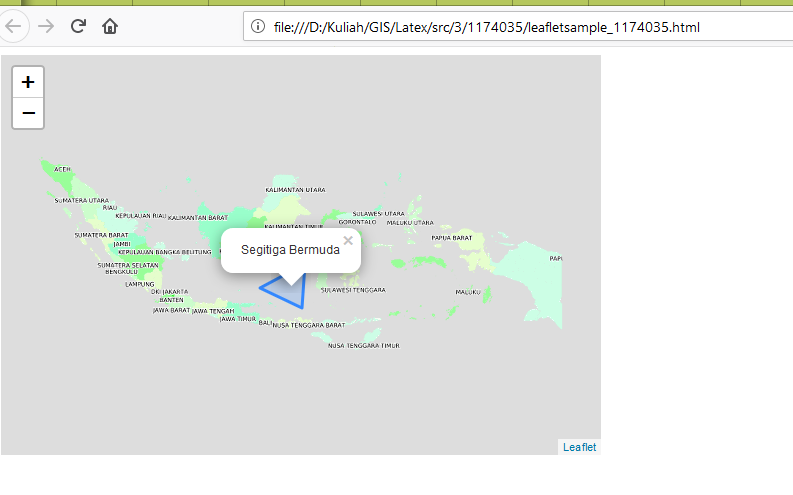
\includegraphics[width=8cm]{figures/1174035/tugas5/6.png}
                \centering
                \caption{Mencoba polygon}
            \end{figure}
            \item Event \break Untuk menggunakan event, silahkan coba dengan kode berikut
            \lstinputlisting[firstline=36, lastline=46]{src/3/1174035/leafletsample_1174035.html}
            \hfill\break
            \begin{figure}[H]
                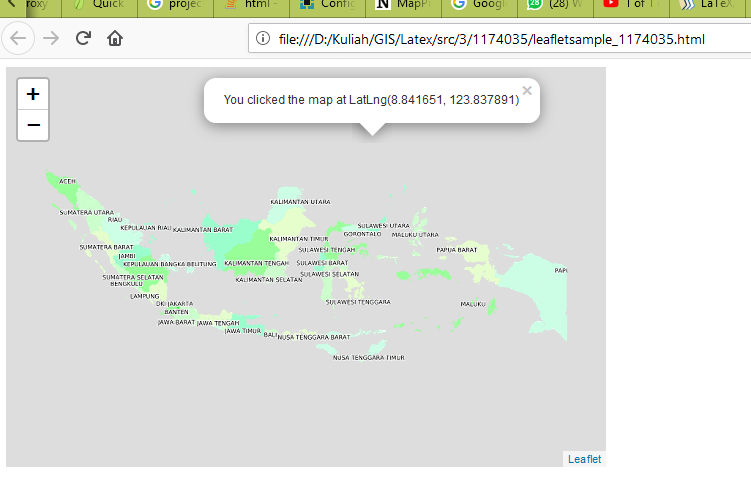
\includegraphics[width=8cm]{figures/1174035/tugas5/7.png}
                \centering
                \caption{Mencoba event}
            \end{figure}
        \end{itemize}
    \item Berikut seluruh kodenya
    \lstinputlisting{src/3/1174035/leafletsample_1174035.html}
    \item Untuk referensi lain bisa dilihat di \href{https://leafletjs.com/}{https://leafletjs.com/}
\end{enumerate}
\subsection{Error Fixing}
Jika peta gak muncul karena file CGI tidak dapat diambil, silahkan ikuti langkah berikut
\begin{enumerate}
    \item Masuk ke directory file MS4W/proj/nad
    \hfill\break
    \begin{figure}[H]
        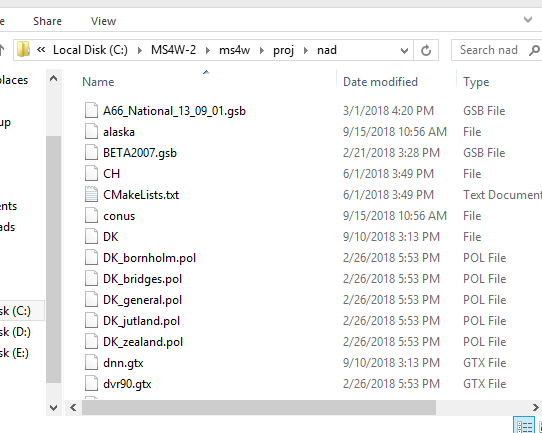
\includegraphics[width=8cm]{figures/1174035/tugas5/error_1.png}
        \centering
        \caption{Mencoba event}
    \end{figure}
    \item Copy Directory tersebut
    \hfill\break
    \begin{figure}[H]
        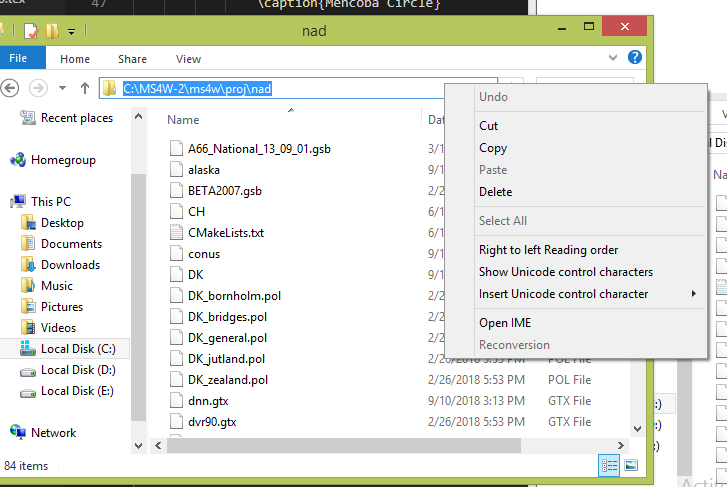
\includegraphics[width=8cm]{figures/1174035/tugas5/error_2.png}
        \centering
        \caption{Mencoba event}
    \end{figure}
    \item Buka file map yang digunakan dan tambahkan kode berikut
    \hfill\break
    \begin{figure}[H]
        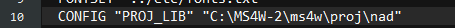
\includegraphics[width=8cm]{figures/1174035/tugas5/error_3.png}
        \centering
        \caption{Mencoba event}
    \end{figure}
\end{enumerate}
\subsection{Cek Plagiarisme}
\hfill\break
\begin{figure}[H]
    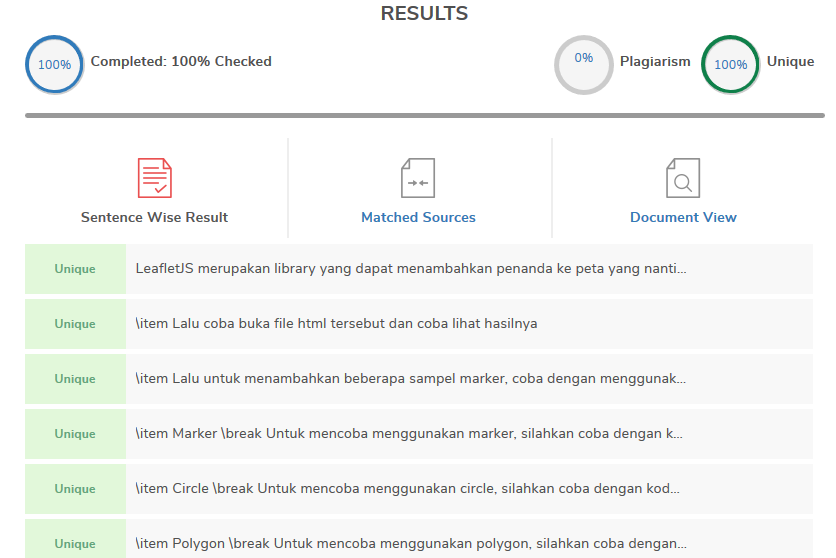
\includegraphics[width=8cm]{figures/1174035/tugas5/plagiarism.png}
    \centering
    \caption{Mencoba event}
\end{figure}
\subsection{Link Youtube}
\href{https://youtu.be/pUeH1U6jcs4}{Tutorial Leaflet JS}